%% Ekstra figures for 1D LSWE other sigma values
\section{Additional figures from 1D LSWE sphere CNN and FNO}\label{app:1D_SWE_spherical_CNN_FNO}
Results for the other sigma values.


CNN, $\sigma = \frac{\pi}{8}$.
\begin{figure}[H]
    \centering
    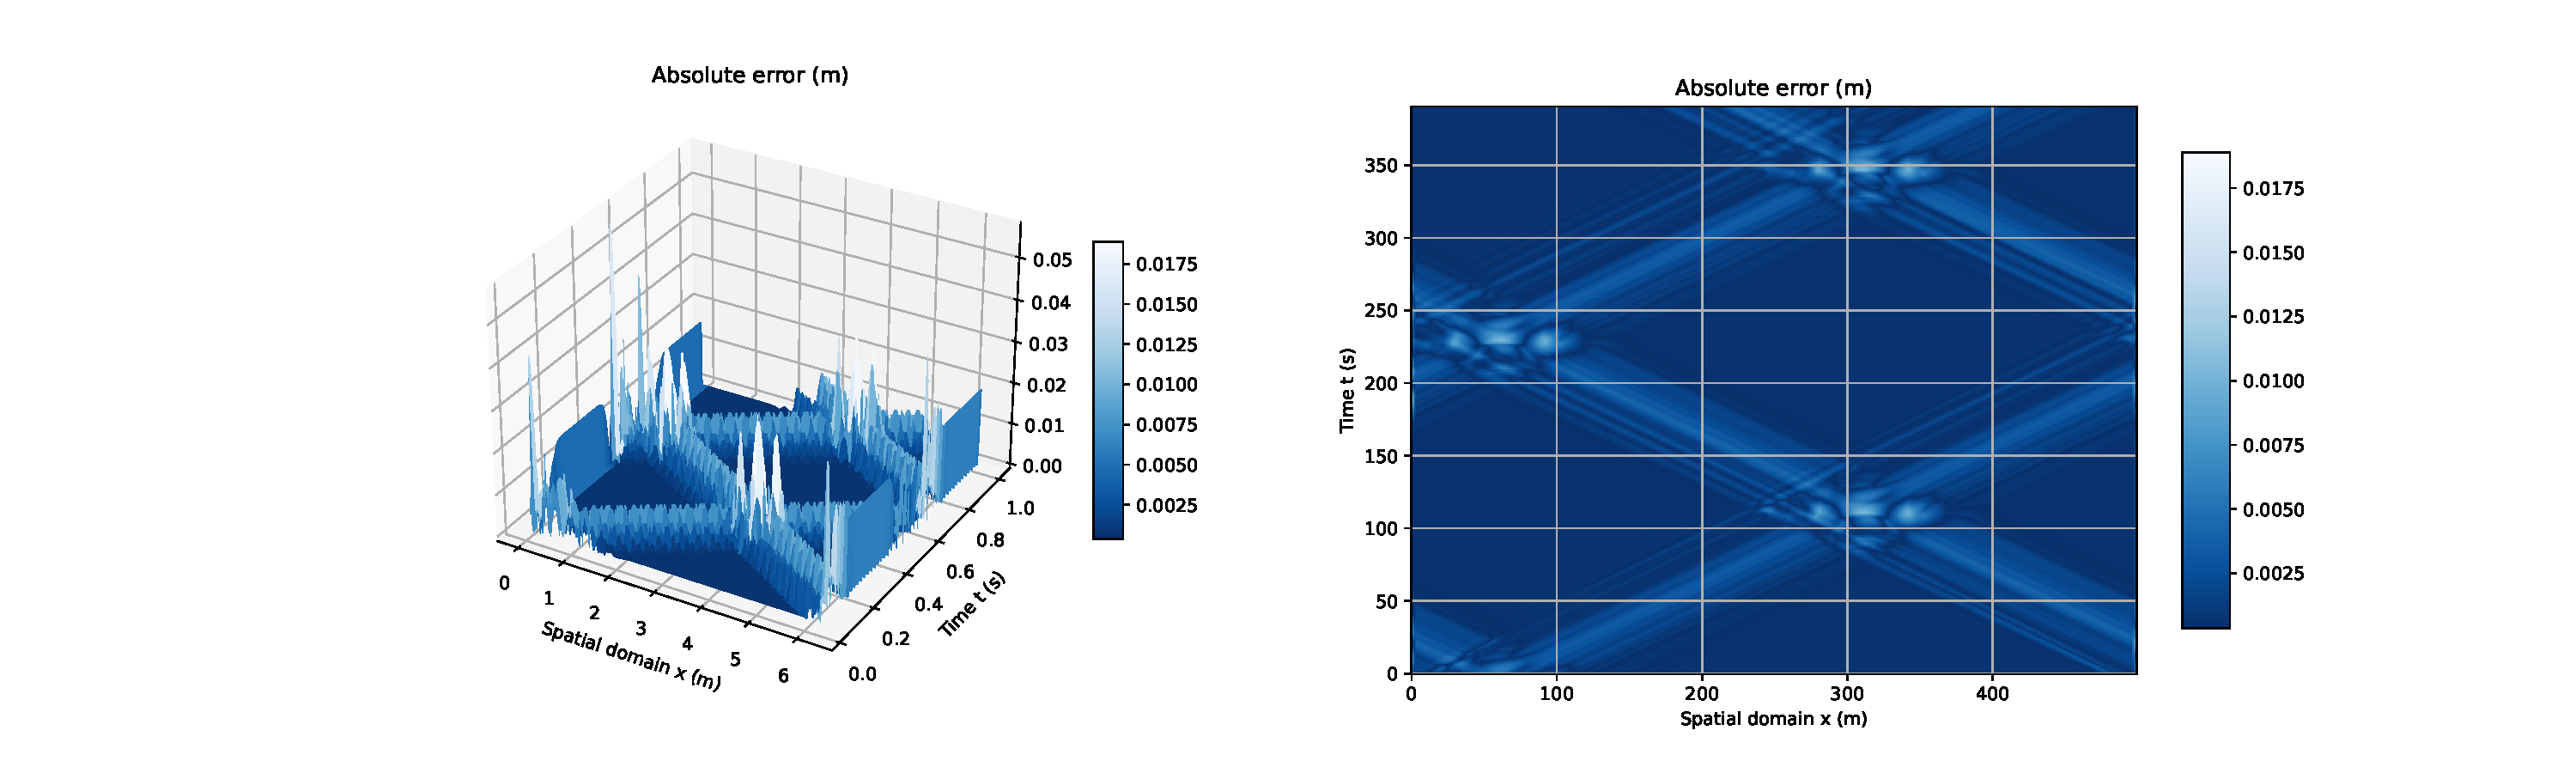
\includegraphics[width=\textwidth]{C:/Users/Matteo/Shallow-Water-Equations/plots/1D_CNN_sphere_error_sigma=1.pdf}
    \caption{Error for the 1D SWE spherical CNN with $\sigma = \frac{\pi}{8}$.}
\end{figure}

\begin{figure}[H]
    \centering
    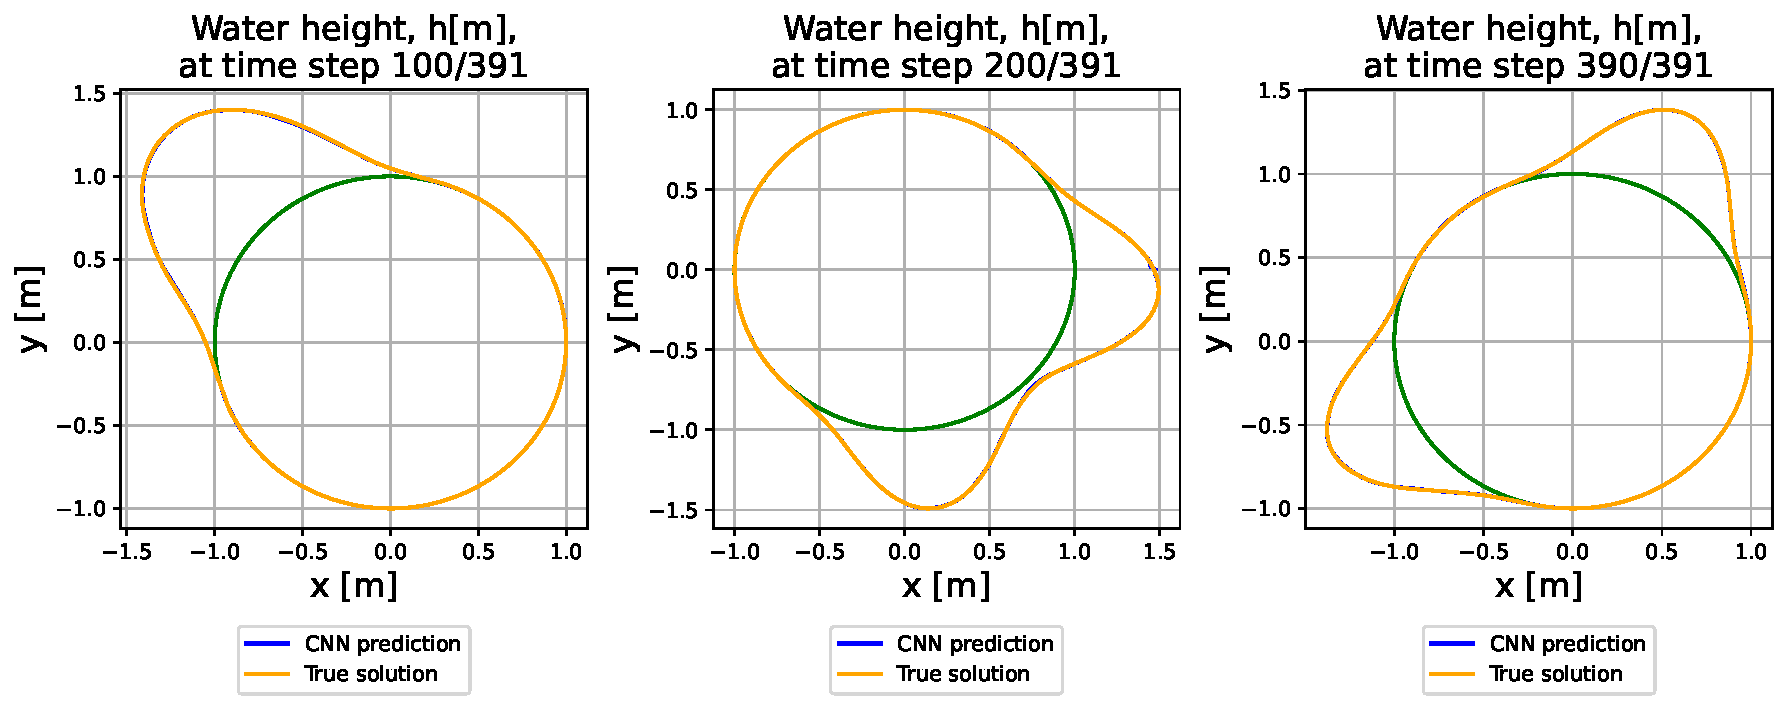
\includegraphics[width=0.9\textwidth]{C:/Users/Matteo/Shallow-Water-Equations/plots/1D_CNN_sphere_pred_timesteps_sphere_sigma=1.pdf}
    \caption{Results for the 1D SWE spherical CNN with $\sigma = \frac{\pi}{8}$.}
\end{figure}

FNO, $\sigma = \frac{\pi}{8}$.
\begin{figure}[H]
    \centering
    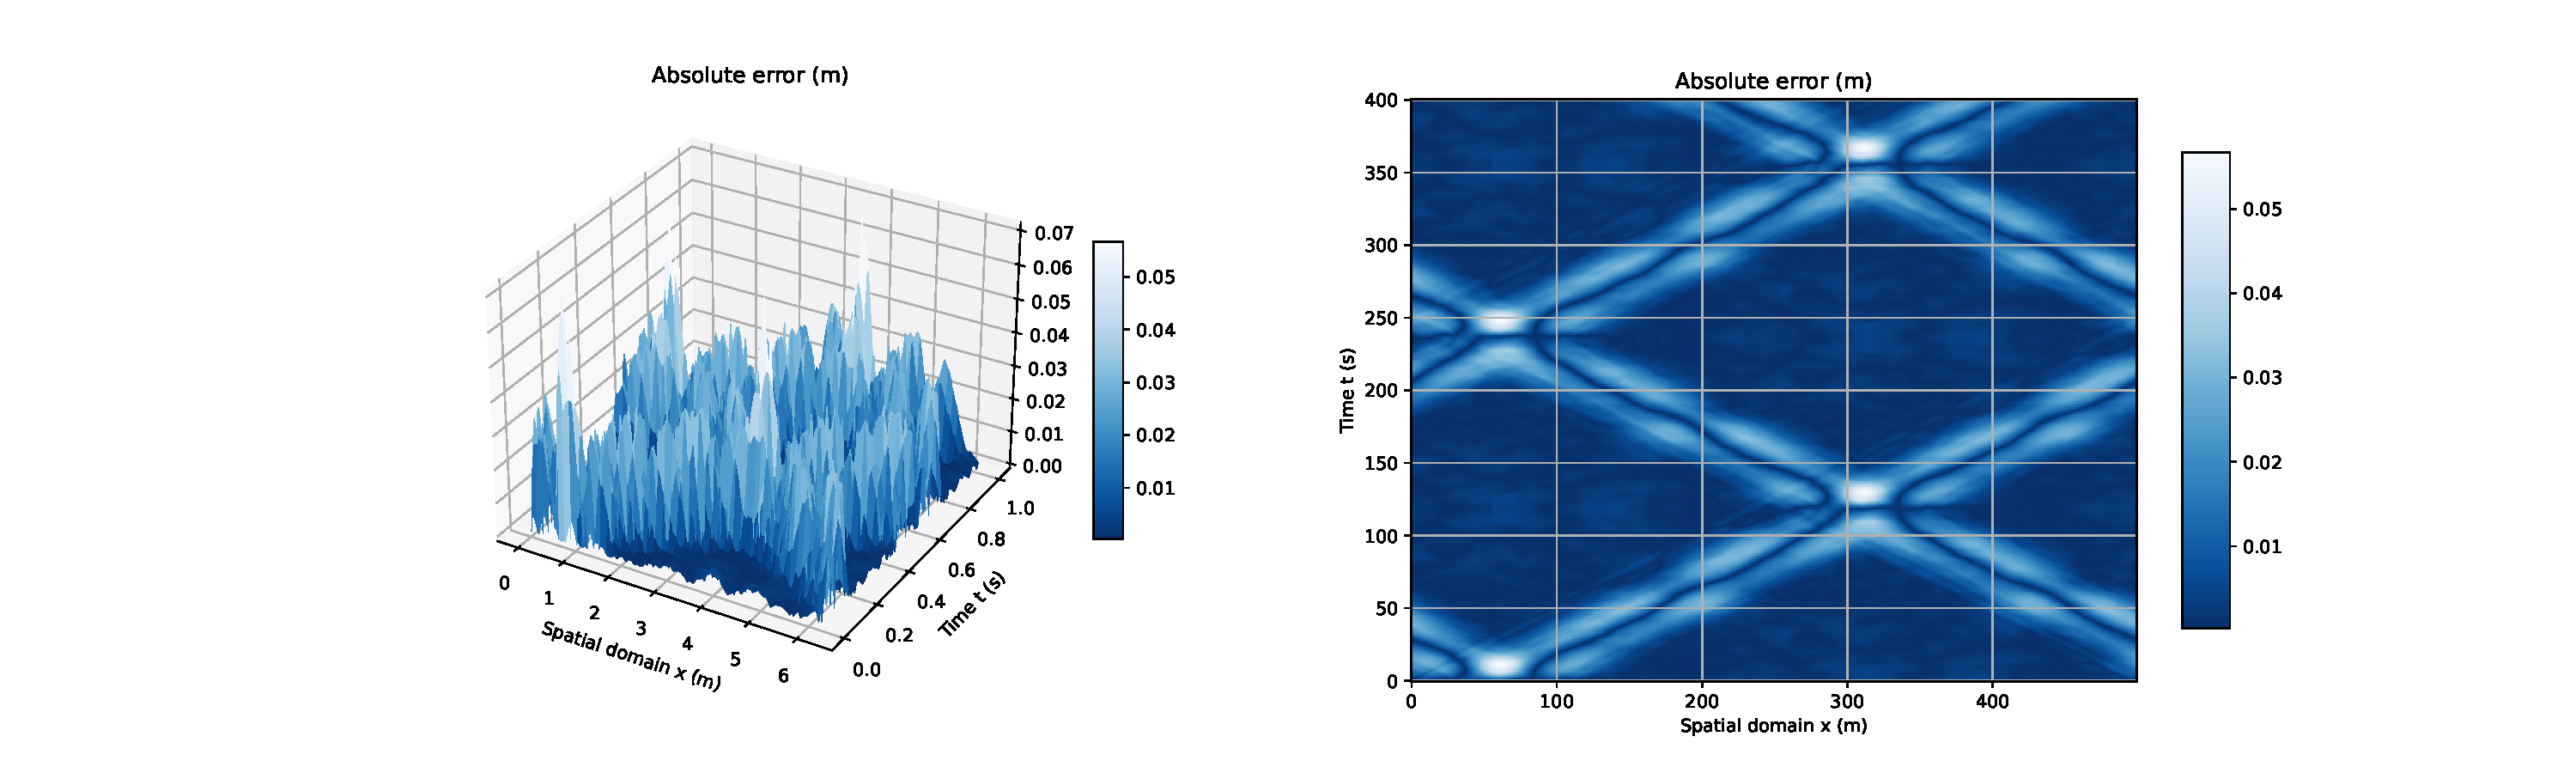
\includegraphics[width=\textwidth]{C:/Users/Matteo/Shallow-Water-Equations/plots/1D_FNO_sphere_error_sigma=1.pdf}
    \caption{Error for the 1D SWE spherical FNO with $\sigma = \frac{\pi}{8}$.}
\end{figure}

\begin{figure}[H]
    \centering
    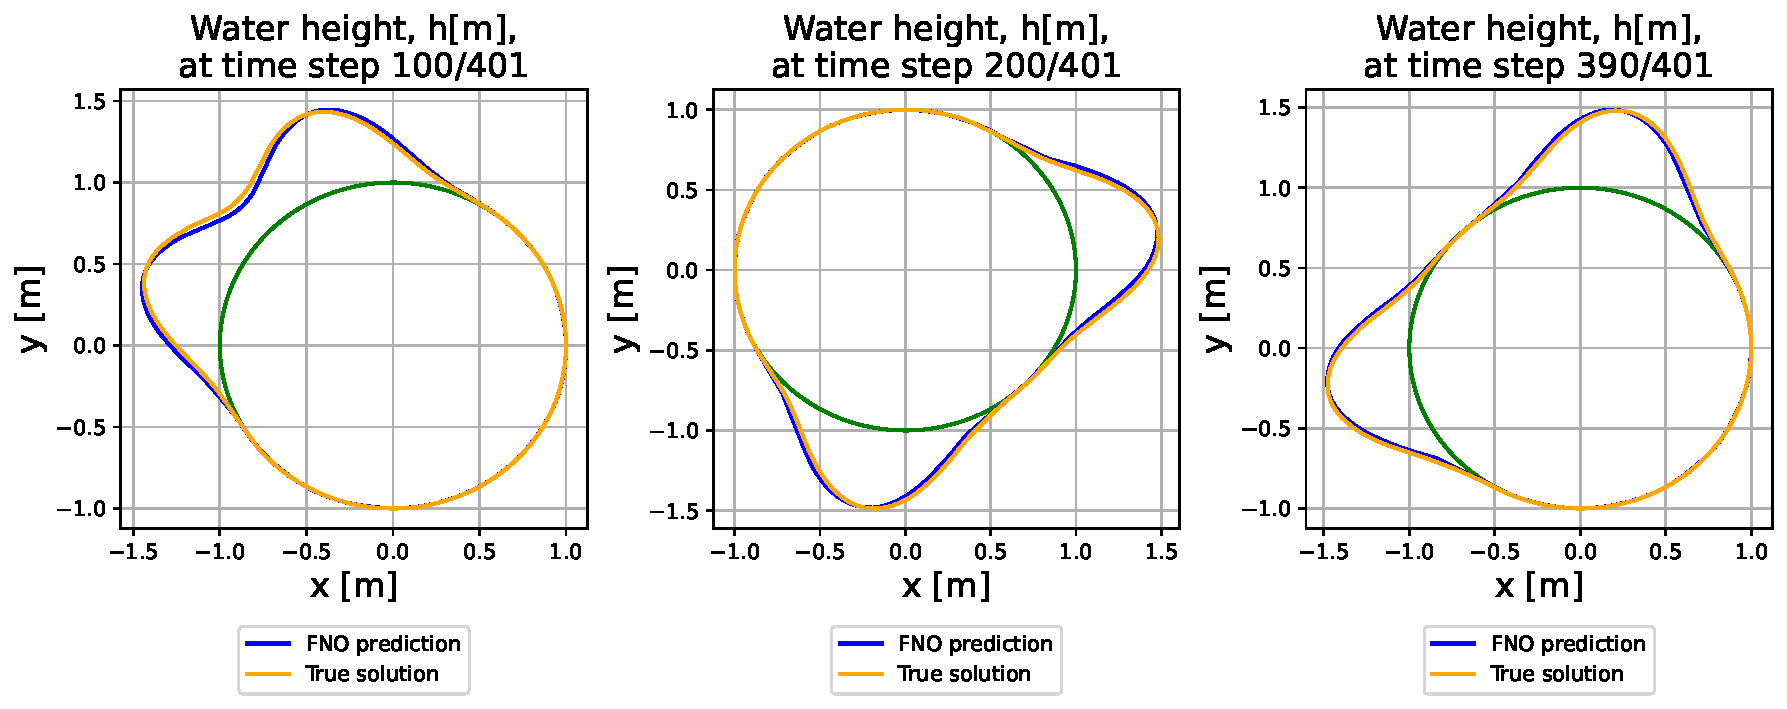
\includegraphics[width=0.9\textwidth]{C:/Users/Matteo/Shallow-Water-Equations/plots/1D_FNO_sphere_pred_timesteps_sphere_sigma=1.pdf}
    \caption{Results for the 1D SWE spherical FNO with $\sigma = \frac{\pi}{8}$.}
\end{figure}

CNN $\sigma = \frac{\pi}{32}$.
\begin{figure}[H]
    \centering
    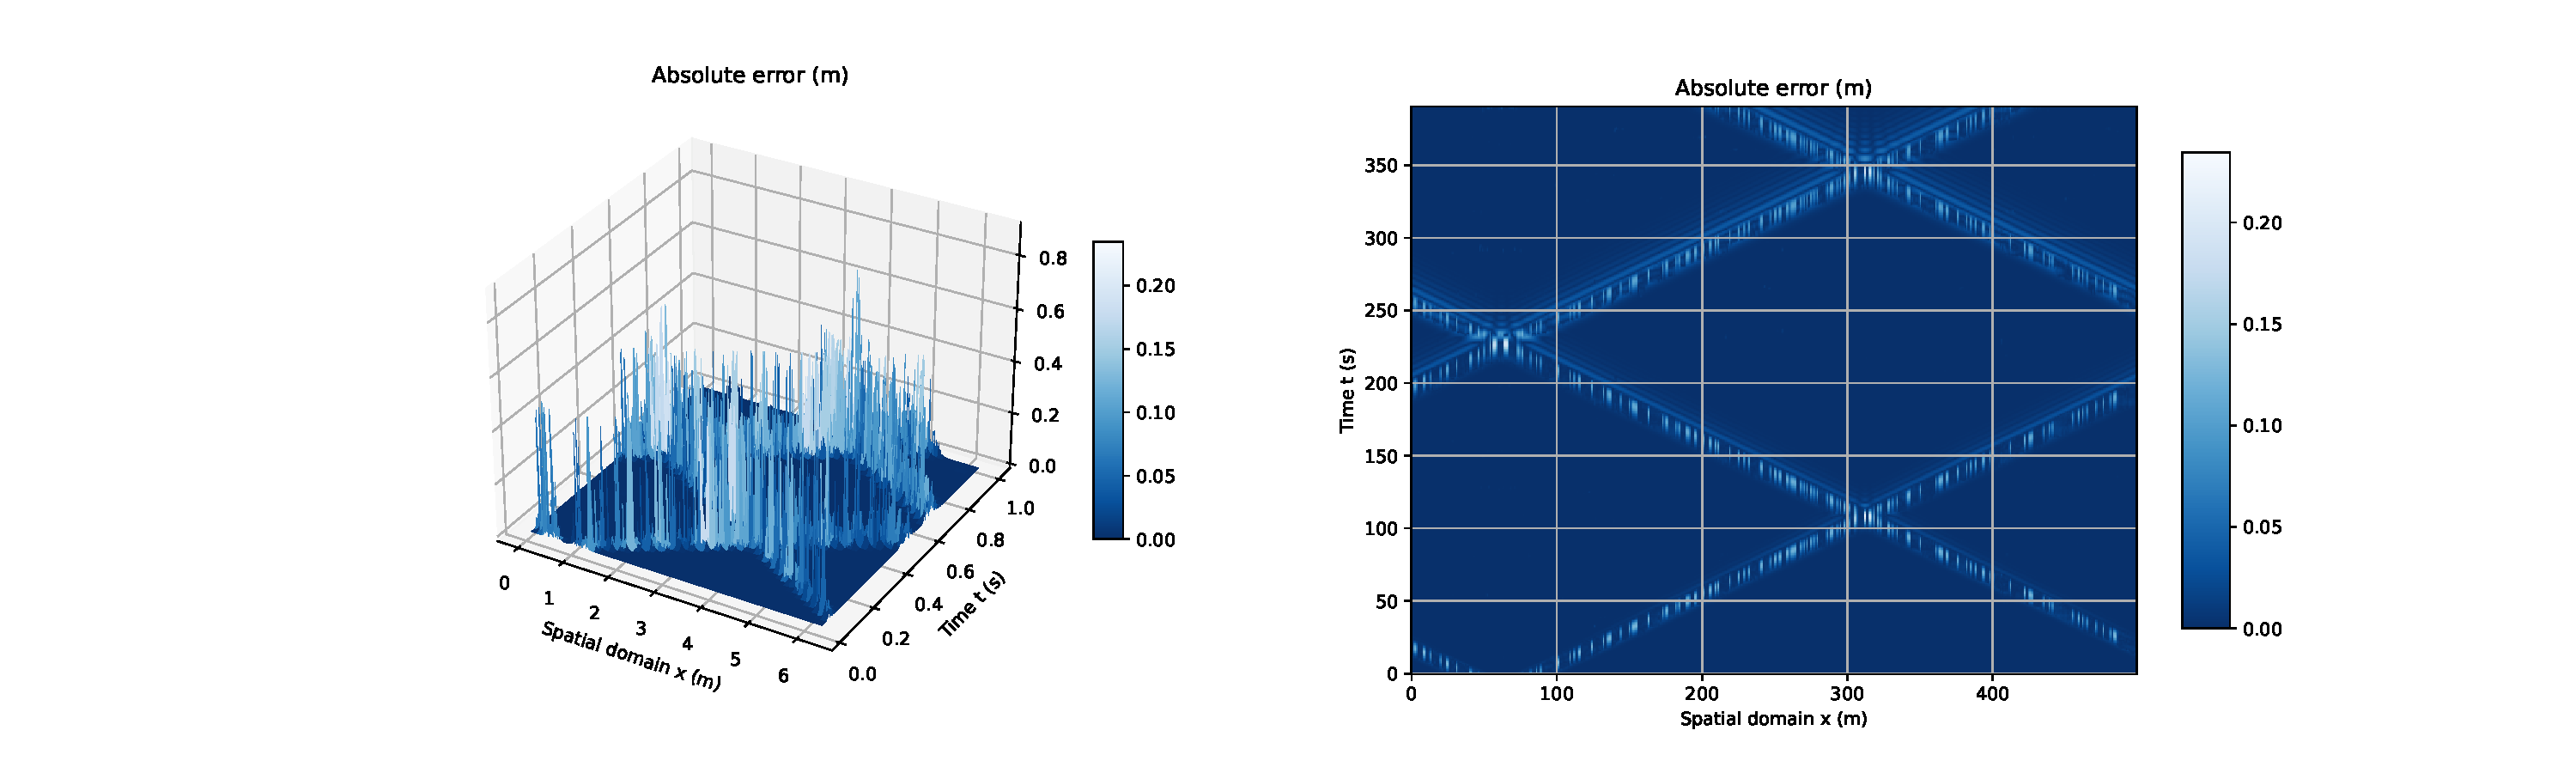
\includegraphics[width=\textwidth]{C:/Users/Matteo/Shallow-Water-Equations/plots/1D_CNN_sphere_error_sigma=3.pdf}
    \caption{Error for the 1D SWE spherical CNN with $\sigma = \frac{\pi}{32}$.}
\end{figure}

\begin{figure}[H]
    \centering
    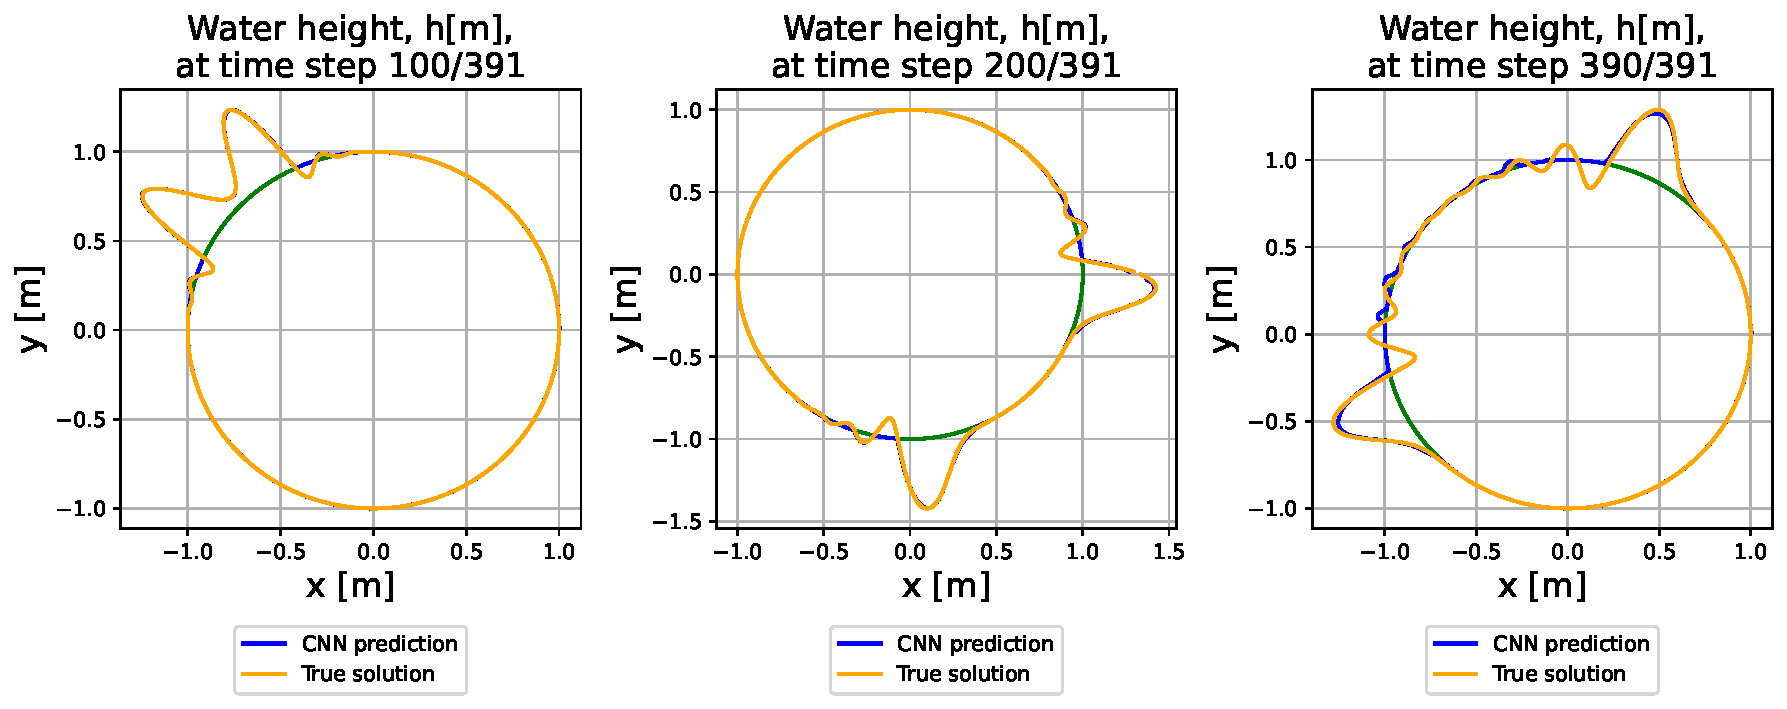
\includegraphics[width=\textwidth]{C:/Users/Matteo/Shallow-Water-Equations/plots/1D_CNN_sphere_pred_timesteps_sphere_sigma=3.pdf}
    \caption{Results for the 1D SWE spherical CNN with $\sigma = \frac{\pi}{32}$.}
\end{figure}


FNO $\sigma = \frac{\pi}{32}$.
\begin{figure}[H]
    \centering
    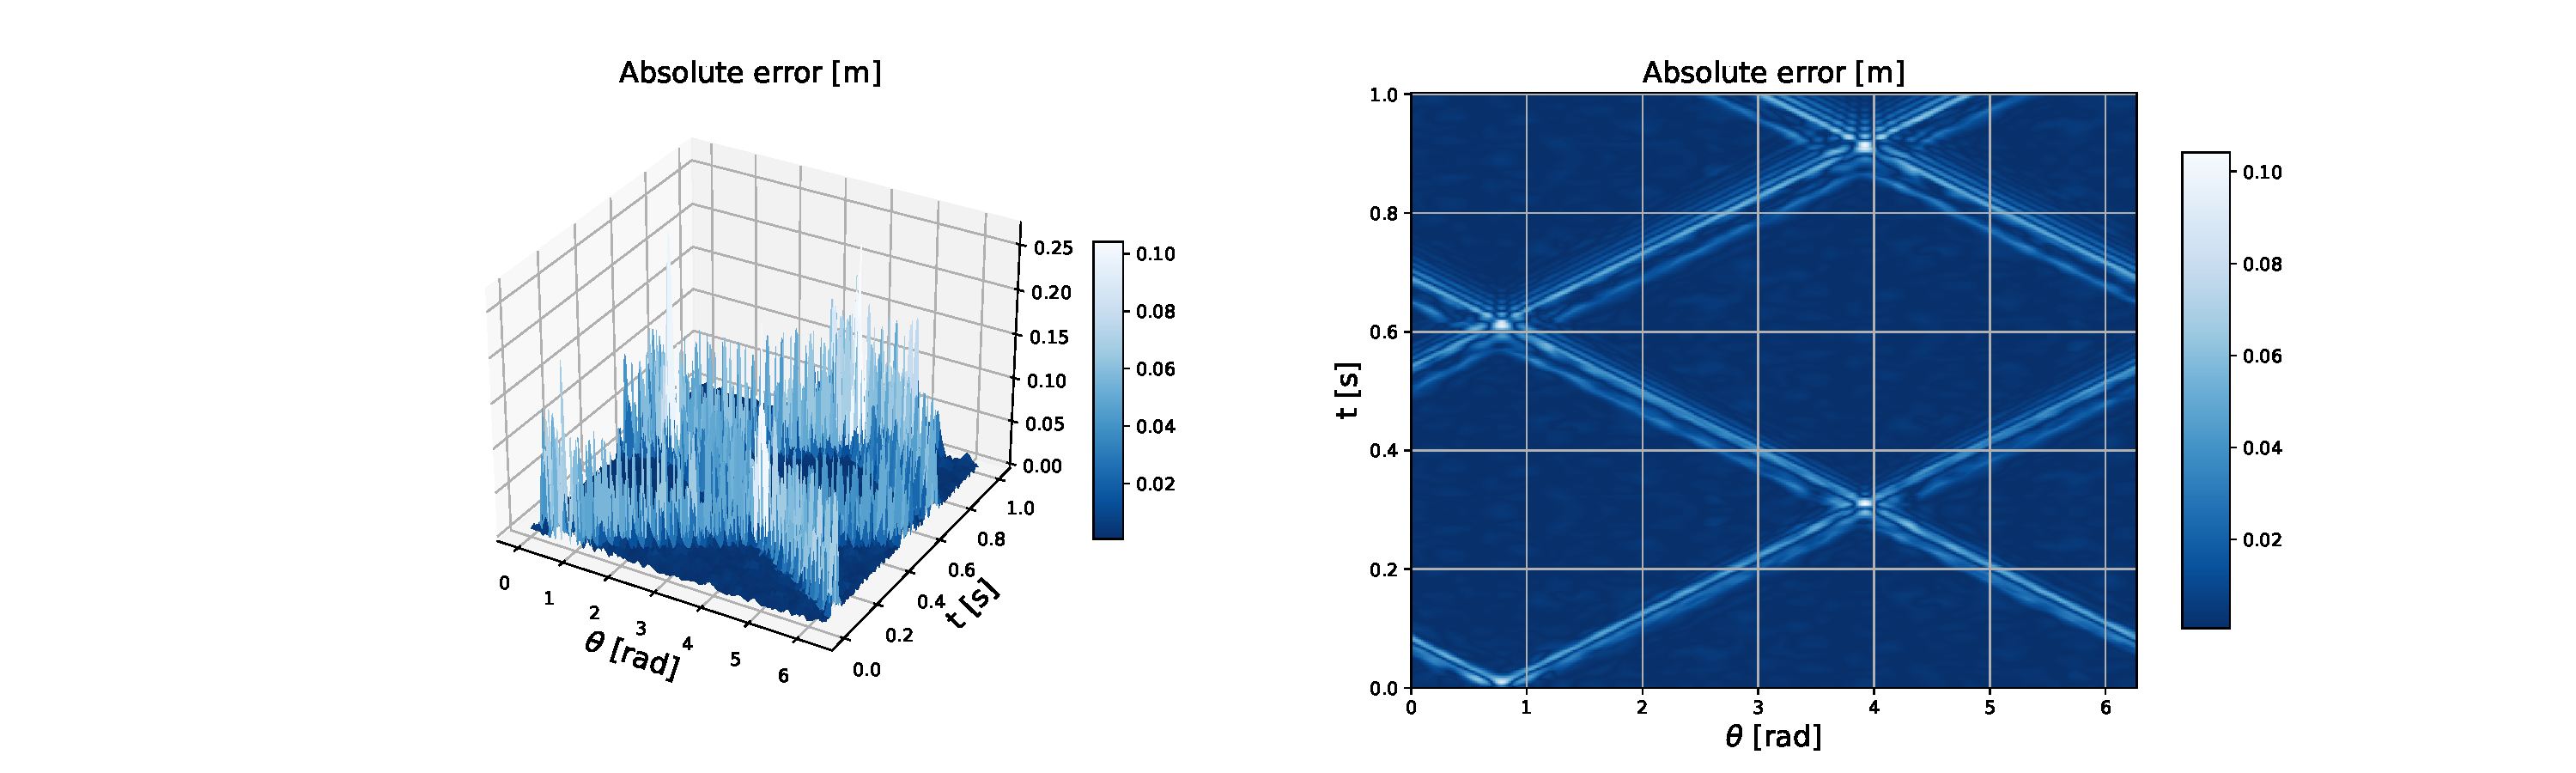
\includegraphics[width=\textwidth]{C:/Users/Matteo/Shallow-Water-Equations/plots/1D_FNO_sphere_error_sigma=3.pdf}
    \caption{Error for the 1D SWE spherical FNO with $\sigma = \frac{\pi}{32}$.}
\end{figure}

\begin{figure}[H]
    \centering
    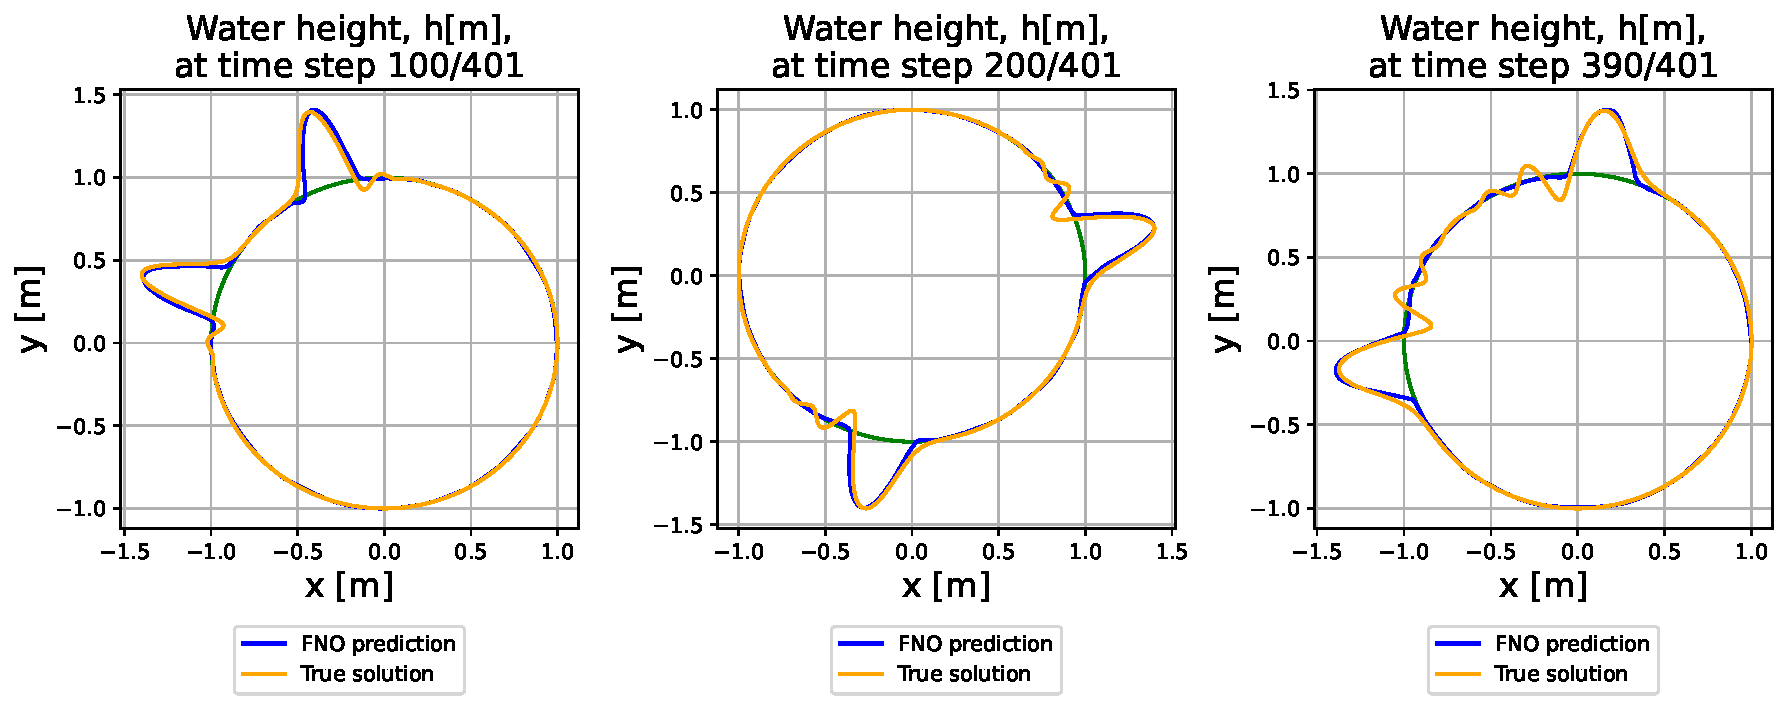
\includegraphics[width=\textwidth]{C:/Users/Matteo/Shallow-Water-Equations/plots/1D_FNO_sphere_pred_timesteps_sphere_sigma=3.pdf}
    \caption{Results for the 1D SWE spherical FNO with $\sigma = \frac{\pi}{32}$.}
\end{figure}





%% Tabellere summary results


\begin{table}[H]
    \centering
    \begin{tabular}{|p{2cm}|c|p{3.3cm}|p{6.2cm}|}
        \hline
        \textbf{Case}  & \textbf{Accuracy} & \textbf{Run time} & \textbf{Features}  \\ \hline
        1D SWE & CNN outperforms FNO. & CNN is faster than FNO. The run time for the FVM is not analysed, as it is very fast (a few seconds). & When presented for a new initial condition, FNO maintained accuracy, where CNO experienced a slight drop in precision. \\ \hline
        1D LSWE on a sphere & CNN outperforms FNO. & CNN is faster than FNO. The run time for the FVM is not analysed, as it is very fast (a few seconds). & For the steepest initial condition, the MSE and MAE for CNN and FNO are almost identical. \\ \hline
    \end{tabular}
    \caption{Summary of the results for the 1D SWE and 1D LSWE on a sphere.} \label{tab:summary_1D}
\end{table}

\begin{table}[H]. 
    \centering
    \begin{tabular}{|c|c|c|p{6.5cm}|}
        \hline
        \textbf{Case}  & \textbf{Accuracy} & \textbf{Run time} & \textbf{Features}  \\ \hline
        2D SWE & FNO shows higher accuracy than the CNN. & CNN is faster than the FNO. 
    \end{tabular}
\end{table}






%% Sphere triangular mesh - fjernet 21.01.2025


We will short outline the proces of the solving the SWE on this grid structure, inspired by the finite element method (FEM).
For simplicity, we will begin by considering the first level of refinement, which consists of 20 triangles.
The matrix tri is a $20 \times 3$ matrix, where each row represents a triangle and the three columns represent the three vertices of the triangle.
The vertices are stored in the matrix $P$, which is a $12 \times 3$ matrix, where each row represents a vertex and the three columns represent the x, y, and z coordinates of the vertex.
The vertices are normalized to the unit sphere, i.e., the radius of the sphere is 1.
The idea is now, that similar to the case in cartesian coordinates, we loop through each cell, in this case triangles, and calculate the fluxes between the cells.
We must be aware of which cells/triangles are neighbors, and we must also be aware of the orientation of the triangles, i.e., the normal vector of the triangle.
The normal vector is calculated by the cross product of the two vectors that span the triangle.
The normal vector is then normalized to the unit sphere.
The matrix tri is my Element to Vertex matrix. 
I also need an Element-to-Face table and a Element-to-Element table.
The Element-to-Face table is used to define which edges or faces belong to each triangle.
Each face of a triangle is an edge shared between two triangles.
That is, it indicates which triangles share an edge. This is important when calculating the fluxes between the triangles.
To construct this table we loop through each triangle and check if the edge of the triangle is shared with another triangle.


We make the FVM to solve SWE for a triangular grid on the sphere.
For each triangle, we consider each face (edge).
For each face we define the normal vector in terms of the spherical unit vectors $\mathbf{e}_\theta$ and $\mathbf{e}_\phi$.
The spherical unit vectors at a point are:
\begin{align*}
    \mathbf{e}_\theta &= \begin{bmatrix}
        - \sin(\theta) \\
        \cos(\theta) \\
        0
    \end{bmatrix}, \\
    \mathbf{e}_\phi &= \begin{bmatrix}
        \cos(\phi) \cos(\theta) \\
        \cos(\phi) \sin(\theta) \\
        -\sin(\phi)
    \end{bmatrix}.
\end{align*}
Where $\mathbf{e}_r$ is the radial direction, going outward from the origin.
$\mathbf{e}_\theta$ is the longitude direction, and $\mathbf{e}_\phi$ is the latitude direction.
The unit vectors are tangensial to the sphere.
We do not need to consider the radial direction, as the SWE is only in the tangential directions.

Now we have the cartesian edge vectors in tangential directions, $\mathbf{e}_0, \mathbf{e}_1, \mathbf{e}_2$.

The projection of an edge vector \( \mathbf{e}_i = (e_{ix}, e_{iy}, e_{iz}) \) onto \( \mathbf{e}_\theta \) is:

\[
\mathbf{e}_i \cdot \mathbf{e}_\theta = e_{ix} \left( -\sin \theta \cos \phi \right) + e_{iy} \left( -\sin \theta \sin \phi \right) + e_{iz} \cos \theta
\]

Similarly, the projection onto \( \mathbf{e}_\phi \) is:

\[
\mathbf{e}_i \cdot \mathbf{e}_\phi = e_{ix} \left( -\sin \phi \right) + e_{iy} \cos \phi
\]

Recall that the cross product between two vectors in 3D produces a third vector that is orthogonal to the two input vectors, i.e., the plane spanned by the two input vectors.

For a given face $f$ of a triangle, we first calculate the Cartesian face normal $\mathbf{n}_f$ as the cross product of the two vectors that span the face.
For a given face $f$ of a triangle, we define the normal vector $\mathbf{n}_f$ is decomposed into the spherical unit vectors as










\begin{equation}\label{eq:momentum_conservation_all}
    \left.
    \begin{aligned}
        u_x + v_y + w_z &= 0, \\
        u_t + u u_x + v u_y + w u_z &= - \frac{1}{\rho} p_x, \\
        v_t + u v_x + v v_y + w v_z &= - \frac{1}{\rho} p_y, \\
        w_t + u w_x + v w_y + w w_z &= - \frac{1}{\rho} p_z - g.
    \end{aligned}
    \right\}
\end{equation}

%% Fjernet 19.01.2025
An alternative integral form of~\eqref{eq:vector_form_1D} is stated in~\cite{Toro2024}:
\begin{align}\label{eq:integral_form_1D_alternative}
    \frac{\text{d}}{\text{d}t} \int_{x_L}^{x_R} \mathbf{U}(x,t) \text{ d}x = \mathbf{F}(\mathbf{U}(x_L, t)) - \mathbf{F}(\mathbf{U}(x_R, t)) + \int_{x_L}^{x_R} \mathbf{S}(\mathbf{U}) \text{ d}x.
\end{align}
From~\eqref{eq:integral_form_1D_alternative} we get that the integral form of the homogeneous SWE in 1D is given by
\begin{align}\label{eq:integral_form_1D_homogeneous}
    \frac{\text{d}}{\text{d}t} \int_{x_L}^{x_R} \mathbf{U}(x,t) \text{ d}x = \mathbf{F}(\mathbf{U}(x_L, t)) - \mathbf{F}(\mathbf{U}(x_R, t)),
\end{align}
meaning that the rate of change of the integral over a spatial domain is equal to the net flux through the boundaries of the domain.











\section{Metod of manufactured solutions}
Method of manufactured solutions (MMS) was used to verify the implementation.
We use a manufactured solution for $h(x,t)$ and $u(x,t)$.
Choose a simple sine wave function for the water height $h$ and a corresponding $u$ that satisfies the shallow water equations.
Consider
\begin{align*}
    h(x,t) &= h_0 + A \cos(\omega t - kx), \\
    u(x,t) &= \frac{ A \omega }{k h_0}  \cos(\omega t - kx),
\end{align*} 
where $h_0$ is the constant base depth, $A$ is the amplitude of the wave, $k$ is the wave number, and $\omega$ is the angular frequency.

We begin by computing the source terms $S_h$ and $S_u$.
First we compute the partial derivatives
\begin{align*}
    h_t &= ,\\
    u_t &=  \\
\end{align*}
which gives (using the chain rule)
\begin{align*}
    {(hu)}_x &= h_x u + h u_x \\
    &= 
\end{align*}



\begin{figure}[htbp]
    \centering
    % First row
    \begin{subfigure}[b]{0.4\textwidth}
        \centering
        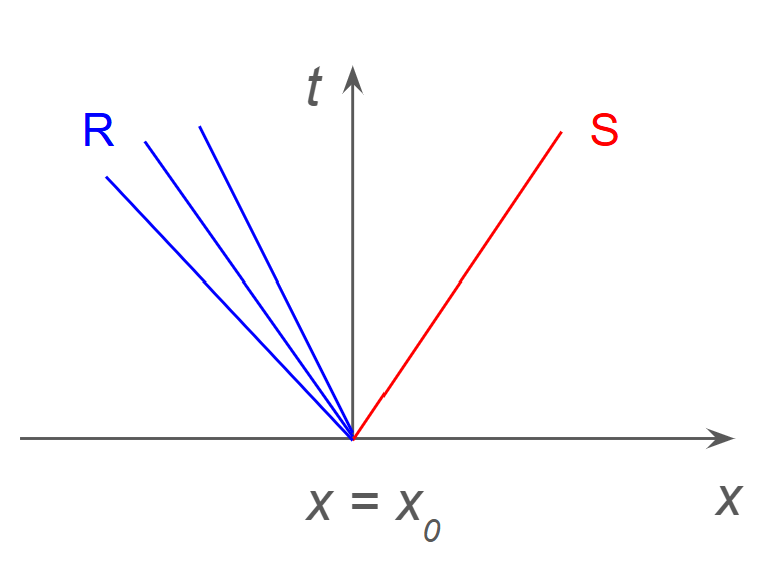
\includegraphics[width=\textwidth]{C:/Users/Matteo/Shallow-Water-Equations/figs/waves-LRRS.png}
        \caption{Left rarefaction wave, right shock wave.}\label{fig:waves-LRRS}
    \end{subfigure}
    \hspace{0.02\textwidth} % Small horizontal space between figures
    \begin{subfigure}[b]{0.4\textwidth}
        \centering
        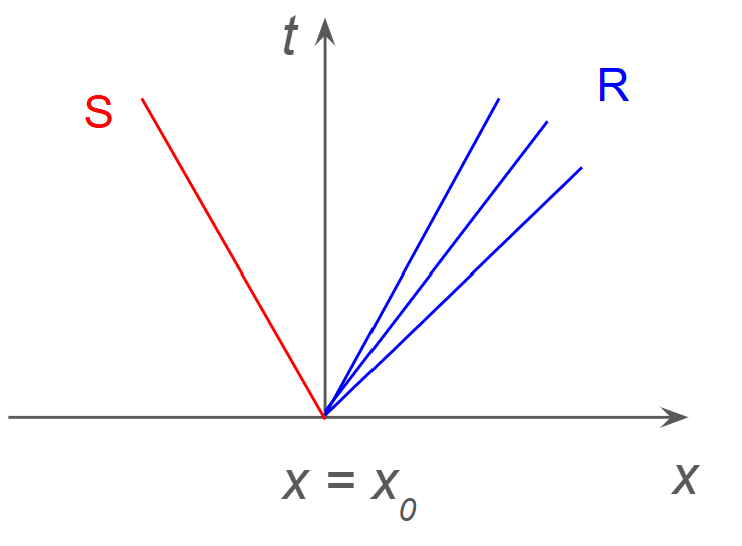
\includegraphics[width=\textwidth]{C:/Users/Matteo/Shallow-Water-Equations/figs/waves-LSRR.png}
        \caption{Left shock wave, right rarefaction wave.}\label{fig:waves-LSRR}
    \end{subfigure}
    
    % Second row
    \begin{subfigure}[b]{0.4\textwidth}
        \centering
        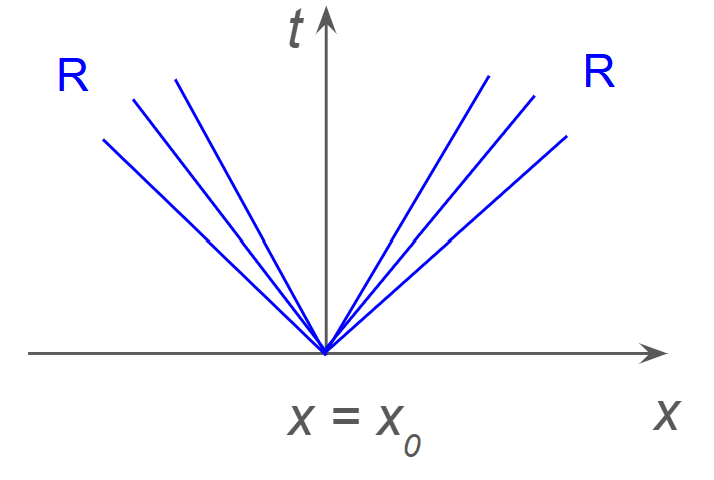
\includegraphics[width=\textwidth]{C:/Users/Matteo/Shallow-Water-Equations/figs/waves-LRRR.png}
        \caption{Left and right rarefaction waves.}\label{fig:waves-LRRR}
    \end{subfigure}
    \hspace{0.02\textwidth} % Small horizontal space between figures
    \begin{subfigure}[b]{0.4\textwidth}
        \centering
        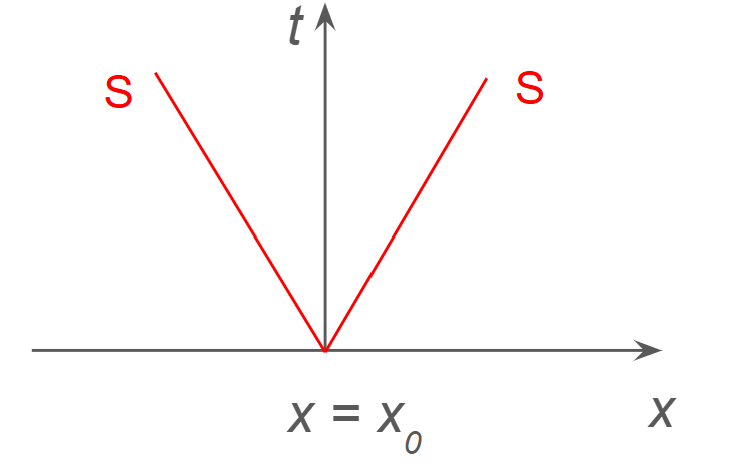
\includegraphics[width=\textwidth]{C:/Users/Matteo/Shallow-Water-Equations/figs/waves-LSRS.png}
        \caption{Left and right shock waves.}\label{fig:waves-LSRS}
    \end{subfigure}
    \caption{Four possible wave patterns in the solution of the Riemann problem.}\label{fig:wave-patterns}
\end{figure}


\subsection{Flux-splitting/Upwind}
In the flux splitting we compute $h_*$ and $u_*$ by assuming a two-rarefaction wave structure.
We define 
\begin{align*}
    c_L = \sqrt{g h_L}, \quad c_R = \sqrt{g h_R},
\end{align*}
to obtain
\begin{align*}
    h_{S2} = {\left( \frac{0.75}{\sqrt{g}} \cdot (q_L - q_R) + 0.5 \cdot \left(h_L^{1.5} + h_R^{1.5}\right) \right)}^2, \\
    h_{S} = h_{S2}^{\frac{1}{3}}
\end{align*}
and
\begin{align*}
    u_* = \frac{1}{2} (u_L + u_R) + \frac{1}{3} \sqrt{g} (h_L^{1.5} - h_R^{1.5}).
\end{align*}




\subsection{Roe solver}
Consider the non-linear Riemann problem in~\eqref{eq:Riemann_problem}:
\begin{align*}
    \mathbf{U}_t + \mathbf{F(U)}_x \equiv \mathbf{U}_t + \mathbf{A} \mathbf{U}_x = 0,
\end{align*}
where $\mathbf{A}$ is the Jacobian matrix of $\mathbf{F}$. 
The Roe solver is based on an approximation of the Jacobian matrix $\mathbf{A}$ by a Roe matrix $\tilde{\mathbf{A}}$, which is a constant coefficient matrix, to obtain the linear system
\begin{align*}
    \mathbf{U}_t + \mathbf{\tilde{A}} \mathbf{U}_x = 0.
\end{align*}

This means that the Roe solver solves the approximated Riemann problem
\begin{align*}
    \mathbf{U}_t + \mathbf{\tilde{A}} \mathbf{U}_x &= 0. \\
    \mathbb{U}(x,0) = \begin{cases}
        \mathbf{U}_L, & x < 0, \\
        \mathbf{U}_R, & x > 0.
    \end{cases}
\end{align*}
exact.
That is, the original non-linear conservation laws are replaced by a linearised system with constant coefficients.

The main idea in the Roe solver is to find average values $\tilde{h}, \tilde{a}, \tilde{u}$ and $\tilde{\psi}$ for the depth $h$, the celerity $a$ (??), the velocity component $u$ and the scalar $\psi$.
The method thus use the following Roe averages:
\begin{align}\label{eq:Roe_averages}
    \left\{
\begin{aligned}
    \tilde{h} &= \sqrt{h_L h_R}, \\
    \tilde{u} &= \frac{u_L \sqrt{h_L} + u_R \sqrt{h_R}}{\sqrt{h_L} + \sqrt{h_R}}, \\
    \tilde{a} &= \sqrt{\frac{1}{2}(a_L^2 + a_R^2)}, \\
    \tilde{\psi} &= \frac{\psi_L \sqrt{h_L}  + \psi_R \sqrt{h_R}}{\sqrt{h_L} + \sqrt{h_R}}.
\end{aligned}
\right.
\end{align}
The average eigenvalues (of what?) are
\begin{align*}
    \tilde{\lambda}_1 = \tilde{u} - \tilde{a}, \quad \tilde{\lambda}_2 = \tilde{u}, \quad \tilde{\lambda}_3 = \tilde{u} + \tilde{a}, \\
\end{align*} 
with the correspinding right eigenvectors
\begin{align*}
    \tilde{\mathbf{R}}^{(1)} = \begin{bmatrix}
        1 \\ \tilde{u} - \tilde{a} \\ \tilde{\psi}
    \end{bmatrix}, \quad
    \tilde{\mathbf{R}}^{(2)} = \begin{bmatrix}
        0 \\ 0 \\  1
    \end{bmatrix}, \quad
    \tilde{\mathbf{R}}^{(3)} = \begin{bmatrix}
        1 \\ \tilde{u} + \tilde{a} \\ \tilde{\psi}
    \end{bmatrix}.
\end{align*}
The wave strenghts $\tilde{\alpha}_j$ described by Roe averages are given by
\begin{align}
    \left\{
    \begin{aligned}
        \tilde{\alpha}_1 &= \frac{1}{2} \left[ \Delta h - \frac{\tilde{h}}{\tilde{a}} \Delta u  \right], \\
        \tilde{\alpha}_2 &= \frac{1}{2} \left[ \tilde{h} \Delta \psi  \right], \\
        \tilde{\alpha}_3 &= \frac{1}{2} \left[ \Delta h + \frac{\tilde{h}}{\tilde{a}} \Delta u  \right].
    \end{aligned}    
    \right.
\end{align}
Applying theory of linear systems with constant coefficients.
The numerical flux is
\begin{align}\label{eq:Roe_flux}
    \mathbf{F}_{i+\frac{1}{2}} = \frac{1}{2} \left( \mathbf{F}_L + \mathbf{F}_R \right) - \frac{1}{2} \sum_{j=1}^3 \tilde{\alpha}_j \left| \tilde{\lambda}_j \right| \tilde{\mathbf{R}}^{(j)}.
\end{align}
The Roe flux~\eqref{eq:Roe_flux} is used in the explicit conservative scheme to solve the SWE in 1D.

Godunov:
Consider the initial-boundary value problem (IBVP) for a system of $N$ nonlinear hyperbolic conservation (balance?) laws     
\begin{equation}\label{eq:IBVP_system}
    \begin{cases}
    \text{PDEs: }    &\mathbf{U}_t + \mathbf{F(U)}_x = \mathbf{S(U)}, \quad x \in [a, b], \quad t > 0, \\
    \text{ICs: }    &\mathbf{U}(x,0) = \mathbf{U}^{(0)}(x), \quad x \in [a,b], \\
    \text{BCs: }    &\mathbf{U}(a,t) = \mathbf{B}_{L}(t), \quad \mathbf{U}(b,t) = \mathbf{B}_{R}(t), \quad t \geq 0.
    \end{cases}
\end{equation}
The vectors $\mathbf{B}_L (t)$ and $\mathbf{B}_R (t)$ denote the boundary conditions at the left and right boundaries, respectively.
The Godunov Upwind method in conservative form~\eqref{eq:explicit_conservative_1D_SWE} solves the IBVP~\eqref{eq:IBVP_system}.
We compute $h_*$ and $u_*$ by starting with a two-rarefaction wave structure, and solve the wetbed problem iteratively.


Derive FVM scheme 1D SWE spherical:




\begin{align}
    \int_{\theta_L}^{\theta_R} h_t + \frac{H}{r \cos(\phi)} u_\theta \text{ d}\theta = 0 \\
    \int_{\theta_L}^{\theta_R} h_t \text{ d}\theta + \int_{\theta_L}^{\theta_R} \frac{H}{r \cos(\phi)} u_\theta \text{ d}\theta = 0.
\end{align}
Then we integrate the momentum equation in~\eqref{eq:linearized_swe_spherical} over $\theta$ from $\theta_L$ to $\theta_R$ to obtain
\begin{align*}
    \int_{\theta_L}^{\theta_R} u_t \text{ d}\theta + \int_{\theta_L}^{\theta_R} g h_\theta \text{ d}\theta + \int_{\theta_L}^{\theta_R} fu \text{ d} \theta = 0.
\end{align*}


The first term is 
\begin{align*}
    \frac{\partial}{\partial t} \int_{\theta_L}^{\theta_R} h \text{ d}\theta =  \Delta \theta h_t,
\end{align*}
meaning that the first term is the rate of change of the water height $h$ in the control volume.
The second term is
\begin{align*}
    \int_{\theta_L}^{\theta_R} \frac{H}{r \cos(\phi)} u_\theta \text{ d}\theta = \frac{H}{r \cos(\phi)} (u_R - u_L),
\end{align*}
where $u_R$ and $u_L$ are the velocities at the right and left boundaries of the control volume, respectively.



The first term gives the time rate of change in the velocity $u$ in the control volume:
\begin{align*}
    \frac{\partial}{\partial t} \int_{\theta_L}^{\theta_R} u \text{ d}\theta = \Delta \theta u_t.
\end{align*}
The second term gives 
\begin{align*}
    \int_{\theta_L}^{\theta_R} g h_\theta \text{ d}\theta = g(h_R - h_L),
\end{align*}
where $h_R$ and $h_L$ are the heights at the right and left boundaries of the control volume, respectively.
The third term with the Coriolis force gives
\begin{align*}
    \int_{\theta_L}^{\theta_R} fu \text{ d}\theta = f(u_R - u_L) \Delta \theta.
\end{align*} 
Hence, the integral form of the linearized shallow water equations in spherical coordinates with one spatial dimension and time is

Then we integrate~\eqref{eq:integral_form_spherical_1D} over time from $t_1:= t_n$ to $t_2:= t_{n+1}$:
\begin{equation}
    \begin{aligned}
        \int_{t_1}^{t_2} \int_{\theta_L}^{\theta_R} h_t \text{ d}\theta \text{d}t + \int_{t_1}^{t_2} \frac{H}{r \cos(\phi)} (u_R - u_L) \text{ d}t &= 0, \\
        \int_{t_1}^{t_2} \int_{\theta_L}^{\theta_R} u_t \text{ d}\theta \text{d}t + \int_{t_1}^{t_2} g(h_R - h_L) \text{ d}t + \int_{t_1}^{t_2} f(u_R - u_L) \Delta \theta &= 0.
    \end{aligned}
\end{equation}
which equals
\begin{equation}\label{eq:integral_form_spherical_1D_2}
    \begin{aligned}
        \int_{\theta_L}^{\theta_R} h(\theta, t_2) \text{ d}\theta &= \int_{\theta_L}^{\theta_R} h(\theta, t_1) \text{ d}\theta - \frac{H}{r \cos(\phi)} (u_R - u_L) \Delta t, \\
        \int_{\theta_L}^{\theta_R} u(\theta, t_2) \text{ d}\theta &= \int_{\theta_L}^{\theta_R} u(\theta, t_1) \text{ d}\theta - g(h_R - h_L) \Delta t - f(u_R - u_L) \Delta \theta \Delta t.
    \end{aligned}
\end{equation}
We divide~\eqref{eq:derive_integral_form_1D_2} with the cell length $\Delta \theta$ to obtain 
\begin{equation}\label{eq:derive_integral_form_spherical}
    \begin{aligned}
        \frac{1}{\Delta \theta} \int_{\theta_L}^{\theta_R} h(\theta, t_2) \text{ d}\theta &= \frac{1}{\Delta \theta} \int_{\theta_L}^{\theta_R} h(\theta, t_1) \text{ d}\theta -  \frac{\Delta t}{\Delta \theta} \frac{H}{r \cos(\phi)} (u_R - u_L), \\
        \frac{1}{\Delta \theta} \int_{\theta_L}^{\theta_R} u(\theta, t_2) \text{ d}\theta &= \frac{1}{\Delta \theta} \int_{\theta_L}^{\theta_R} u(\theta, t_1) \text{ d}\theta - \frac{\Delta t}{\Delta \theta} g(h_R - h_L)  - f(u_R - u_L) \Delta t.
    \end{aligned}
\end{equation}
By inserting the cell averages in~\eqref{eq:derive_integral_form_spherical}, we obtain the finite volume scheme for the linearized shallow water equations in spherical coordinates with one spatial dimension and time:
\begin{equation}
    \left.
    \begin{aligned}
        h_i^{n+1} &= h_i^n - \frac{\Delta t}{\Delta \theta} (F_{h, i + \frac{1}{2}} - F_{h, i - \frac{1}{2}}),  \\
        u_i^{n+1} &=  u_i^n - \frac{\Delta t}{\Delta \theta} (F_{u, i + \frac{1}{2}} - F_{u, i - \frac{1}{2}}) - \Delta t f(u_{i}^n).
    \end{aligned}
    \right\}
\end{equation}
Where:
\begin{equation}
    \begin{aligned}
        h_i^n &= \frac{1}{\Delta \theta} \int_{\theta_{i-1/2}}^{\theta_{i+1/2}} h(\theta, t_n) \text{ d}\theta, \\
        u_i^n &= \frac{1}{\Delta \theta} \int_{\theta_{i-1/2}}^{\theta_{i+1/2}} u(\theta, t_n) \text{ d}\theta, \\
        F_{h, i + \frac{1}{2}} &= \frac{H}{r \cos(\phi)} (u_{i+1} - u_i), \\
        F_{h, i - \frac{1}{2}} &= \frac{H}{r \cos(\phi)} (u_{i} - u_{i-1}), \\
        F_{u, i + \frac{1}{2}} &= g(h_{i+1} - h_i).
    \end{aligned}
\end{equation}


Now that we have the integral form, we will obtain the finite volume scheme for the linearized shallow water equations in spherical coordinates, by dividing the integral form~\eqref{eq:integral_form_spherical_1D} by the cell length $\Delta \theta$:
\begin{equation}
    \left.
    \begin{aligned}
        h_t + \frac{H}{r \cos(\phi)} \frac{(u_R - u_L)}{\Delta \theta} &= 0, \\
        u_t +  \frac{g (h_R - h_L)}{\Delta \theta} + f(u_R - u_L) &= 0.
    \end{aligned}
    \right\}
\end{equation}


Putting it all together we thus have:
\begin{equation}
    \begin{aligned}
        \Delta \theta h_t + \frac{H}{r \cos(\phi)} (u_R - u_L) &= 0, \\
        \Delta \theta u_t + g(h_R - h_L) + f(u_R - u_L) \Delta \theta &= 0.
    \end{aligned}
\end{equation}
Rewritten as the discretized equations:
\begin{equation}
    \left.
    \begin{aligned}
        h_t &= - \frac{H}{r \cos(\phi)} \frac{(u_R - u_L)}{\Delta \theta}, \\
        u_t &= - \frac{g (h_R - h_L)}{\Delta \theta}  - f(u_R - u_L).
    \end{aligned}
    \right\}
\end{equation}    
Then we calculate the fluxes at the boundaries of the control volume.
In this case we use the most simple fluxes, the average of the velocities at the boundaries, i.e., for cell $i$:
\begin{equation}
    \begin{aligned}
        h_R &= \frac{1}{2} (h_{i+1} + h_i), \\
        h_L &= \frac{1}{2} (h_i + h_{i-1}), \\
        u_R &= \frac{1}{2} (u_{i+1} + u_i), \\
        u_L &= \frac{1}{2} (u_i + u_{i-1}).
    \end{aligned}
\end{equation}
Finally we integrate with respect to time to obtain the finite volume scheme for the linearized shallow water equations in spherical coordinates:
When discretizing the equations, we define the cell averages $h_i^n$ and $u_i^n$ as the average values of the height and velocity in the $i$-th cell at time $t_n$:

Numerical flux\ldots

Time integration.



